% ============================================================================
%  ANN-based Fault Detection and Diagnosis of Induction Motors
%  IEEE conference format. On Overleaf (or any full TeX Live) the real IEEEtran
%  class is used automatically; otherwise ieeelike.sty gives a close look-alike.
% ============================================================================
\IfFileExists{IEEEtran.cls}
  {\documentclass[conference]{IEEEtran}}
  {\documentclass[10pt,twocolumn,letterpaper]{article}\usepackage{ieeelike}}
\usepackage{amsmath,amssymb}
\usepackage{graphicx}
\usepackage{booktabs}
\usepackage{multirow}
\usepackage{cite}
\usepackage{xcolor}
\usepackage{tikz}
\usetikzlibrary{positioning,arrows.meta}
\usepackage{balance}
\usepackage{stfloats}
\usepackage[hidelinks]{hyperref}
\graphicspath{{figs/}}
\setlength{\textfloatsep}{8pt plus 2pt minus 2pt}
\setlength{\floatsep}{6pt plus 2pt minus 2pt}
\setlength{\dbltextfloatsep}{8pt plus 2pt minus 2pt}
\renewcommand{\topfraction}{0.9}\renewcommand{\dbltopfraction}{0.9}\renewcommand{\textfraction}{0.07}\renewcommand{\floatpagefraction}{0.8}\renewcommand{\dblfloatpagefraction}{0.8}

\begin{document}

\title{Artificial Neural Networks for Fault Detection and Diagnosis of Induction Motors Using Simulated Motor Current Signature Analysis}

\author{
\IEEEauthorblockN{Mhamad Naser Dine}
\IEEEauthorblockA{Faculty of Engineering (ESIB)\\ Saint Joseph University of Beirut\\ Beirut, Lebanon}
\and
\IEEEauthorblockN{Ali Srour}
\IEEEauthorblockA{Faculty of Engineering (ESIB)\\ Saint Joseph University of Beirut\\ Beirut, Lebanon}
\and
\IEEEauthorblockN{Supervisor: Hadi Y. Kanaan}
\IEEEauthorblockA{HDR, Ph.D., Eng.\\ Course: AI-Based Control Systems\\ Saint Joseph University of Beirut}
}

\maketitle

\begin{abstract}
Induction motors drive most industrial processes, and their unexpected failure causes costly downtime. This paper presents a complete, simulation-based pipeline for detecting and diagnosing induction-motor faults from the stator current with artificial neural networks (ANNs). A dynamic $\alpha\beta$ model of a 2.2~kW squirrel-cage motor is solved numerically, and four conditions are injected physically into the model: broken rotor bars, stator inter-turn short circuit, outer-race bearing defect and supply-voltage unbalance, each at three severities. With load variation, parameter spread and sensor noise, 1500 motors are simulated and described by 19 motor-current-signature-analysis (MCSA) features. Seven networks implemented from scratch are compared: Perceptron, ADALINE, multilayer perceptrons (MLPs) trained by back-propagation, with momentum, with an adaptive learning rate and with Levenberg--Marquardt, and a radial-basis-function (RBF) network. Training, test (early stopping) and validation sets follow a three-set cross-validation protocol. Over ten independent runs, the back-propagation MLP reaches $94.0\pm1.5$\,\% diagnosis accuracy (five classes), against $93.3$\,\% for the Perceptron and $77.5$\,\% for the RBF network. On 500 unseen motors it recognises incipient faults in 89\,\% of cases and medium or severe faults in 100\,\%. Robustness studies show that the accuracy is maintained within the training noise range but degrades sharply outside it.
\end{abstract}

\begin{IEEEkeywords}
Induction motor, fault diagnosis, motor current signature analysis, multilayer perceptron, back-propagation, Levenberg--Marquardt, RBF network.
\end{IEEEkeywords}

% ----------------------------------------------------------------------------
\section{Introduction}
Three-phase squirrel-cage induction motors are the workhorses of industry: pumps, fans, compressors and conveyors rely on them. Field surveys attribute most of their failures to bearings, stator windings and the rotor cage \cite{nandi2005}. Most faults start small and grow over weeks, so detecting them at an early stage allows maintenance to be planned instead of suffering an unplanned stop.

Motor current signature analysis (MCSA) is attractive for this purpose because it only needs the stator currents, which are often already measured by the drive. Each fault leaves a characteristic signature in the current: sidebands around the supply frequency for broken bars, unbalance and negative-sequence components for winding faults, and components linked to the bearing geometry for bearing defects \cite{benbouzid2000,thomson2001}. Interpreting these signatures by hand requires an expert and fixed thresholds, which fail when faults are small, the load changes or the sensors are noisy. Artificial neural networks can instead learn the decision boundaries from examples \cite{haykin1999,goode1995}.

This work builds a complete pipeline and uses it to compare the neural networks covered in the course. Its contributions are:
\begin{enumerate}
\item a dynamic motor model in which the four fault types are injected \emph{physically} (as parameter changes) rather than as added sine waves;
\item a 19-feature MCSA vector combining time-domain, symmetrical-component, Park's-vector and spectral indicators;
\item from-scratch implementations of seven networks, evaluated with a three-set cross-validation protocol and early stopping;
\item a reliability study: ten repeated runs, robustness to noise, load and severity, and the effect of the hidden-layer size;
\item an interactive Python application (Streamlit) for simulation, training and live diagnosis.
\end{enumerate}

% ----------------------------------------------------------------------------
\section{Methodology Overview}
Fig.~\ref{fig:pipeline} summarises the pipeline. A virtual motor is simulated under a randomly selected condition, severity and load. Its noisy currents and voltages are converted into features, which are normalised and classified by the network. Two tasks are considered: \emph{fault detection} (healthy versus faulty, one output neuron) and \emph{fault diagnosis} (five classes, one output neuron per class).

\begin{figure}[!t]
\centering
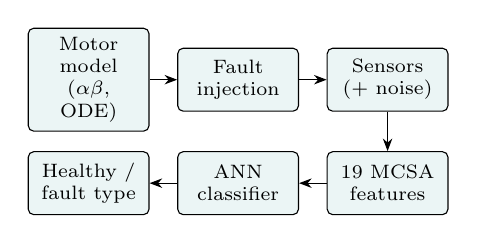
\begin{tikzpicture}[node distance=3mm and 3.5mm, box/.style={draw, rounded corners=2pt, fill=teal!8, align=center, font=\scriptsize, minimum height=8mm, text width=13mm}, >={Stealth[length=1.6mm]}]
\node[box] (m) {Motor model\\($\alpha\beta$, ODE)};
\node[box, right=of m] (f) {Fault\\injection};
\node[box, right=of f] (s) {Sensors\\(+ noise)};
\node[box, below=5mm of s] (x) {19 MCSA\\features};
\node[box, left=of x] (n) {ANN\\classifier};
\node[box, left=of n] (o) {Healthy /\\fault type};
\draw[->] (m) -- (f); \draw[->] (f) -- (s); \draw[->] (s) -- (x); \draw[->] (x) -- (n); \draw[->] (n) -- (o);
\end{tikzpicture}
\caption{Proposed fault detection and diagnosis pipeline.}
\label{fig:pipeline}
\end{figure}

% ----------------------------------------------------------------------------
\section{Induction Motor Model and Fault Injection}
\subsection{Dynamic Model}
The motor is modelled in the stationary $\alpha\beta$ frame with an isolated star point and the amplitude-invariant Clarke transform \cite{krause2002}. The state vector contains the stator and rotor flux linkages, the mechanical speed and the electrical rotor angle, $\mathbf{x}=[\psi_{s\alpha},\psi_{s\beta},\psi_{r\alpha},\psi_{r\beta},\omega_m,\theta_r]$:
\begin{align}
\dot{\boldsymbol{\psi}}_s &= \mathbf{v}_s - \mathbf{R}_s\,\mathbf{i}_s, \\
\dot{\boldsymbol{\psi}}_r &= -\mathbf{R}_r(\theta_r)\,\mathbf{i}_r + \omega_r\,\mathbf{J}\,\boldsymbol{\psi}_r, \quad \mathbf{J}=\begin{bmatrix}0&-1\\1&0\end{bmatrix},\\
\begin{bmatrix}\boldsymbol{\psi}_s\\ \boldsymbol{\psi}_r\end{bmatrix} &= \mathbf{L}\begin{bmatrix}\mathbf{i}_s\\ \mathbf{i}_r\end{bmatrix},\\
T_e &= \tfrac{3}{2}\,p\,(\psi_{r\beta}\, i_{r\alpha}-\psi_{r\alpha}\, i_{r\beta}),\\
J_m\,\dot{\omega}_m &= T_e - T_L(t) - B\,\omega_m,\qquad \dot{\theta}_r = p\,\omega_m .
\end{align}
The equations are integrated with the adaptive Runge--Kutta solver of SciPy (\texttt{solve\_ivp}, RK45). Each simulation starts from the analytical steady state, and 3~s of signals sampled at 4~kHz are recorded after a 0.4~s settling period. Table~\ref{tab:motor} lists the parameters. The model gives 14.7~N$\cdot$m at 1443~rpm (slip 3.8\,\%) and 4.2~A at rated load.

\begin{table}[!t]
\caption{Motor Parameters}
\label{tab:motor}
\centering\footnotesize
\begin{tabular}{@{}lr@{\hspace{10pt}}lr@{}}
\toprule
Rated power & 2.2 kW & $R_s$ & 2.9 $\Omega$\\
Voltage (Y), frequency & 400 V, 50 Hz & $R_r'$ & 2.2 $\Omega$\\
Pole pairs $p$ & 2 & $L_{ls}=L_{lr}$ & 12.5 mH\\
Rotor bars & 28 & $L_m$ & 360 mH\\
Bearing balls & 9 & $J_m$ & 0.012 kg\,m$^2$\\
\bottomrule
\end{tabular}
\end{table}

\subsection{Fault Models}
Each fault is introduced as a physical change of the model, which then naturally produces its signature (Table~\ref{tab:faults}):
\begin{itemize}
\item \emph{Broken rotor bars (BRB):} $n$ broken bars out of $N$ are represented by a rotor-resistance asymmetry $R_{rq}=R_r(1+k)$, with the commonly used approximation $k=3n/(N-3n)$. In the stator frame the resistance matrix $\mathbf{R}_r(\theta_r)$ then depends on $2\theta_r$, which creates the sidebands $(1\pm2ks)f_s$ \cite{thomson2001,bellini2008}.
\item \emph{Stator inter-turn short circuit (ITSC):} a reduced-turns model is used. Phase $a$ keeps a fraction $(1-\mu)$ of its turns, which modifies its resistance, leakage and magnetising coupling and unbalances the machine \cite{tallam2002}.
\item \emph{Outer-race bearing defect (BRG):} the defect is represented as a load-torque oscillation $T_L=T_{L0}+A\cos(K_b\theta_m)$, with $K_b=\tfrac{N_b}{2}(1-\tfrac{d}{D})=3.58$ (outer-race frequency $f_o=K_b f_r$). It produces current components at $|f_s\pm f_o|$ \cite{schoen1995}.
\item \emph{Supply voltage unbalance (VUNB):} one randomly chosen phase voltage is reduced.
\end{itemize}
To make the data realistic, every simulated motor also receives a $\pm5$\,\% spread on $R_s$ and $R_r$, a small natural rotor/stator asymmetry, 0--1\,\% grid unbalance, a load of 30--110\,\%, Gaussian sensor noise of 0.5--2\,\% of the RMS value, 0.5\,\% sensor gain error and a $\pm2$~rpm speed-sensor error.

\begin{table}[!t]
\caption{Fault Classes and Severity Levels}
\label{tab:faults}
\centering\footnotesize
\begin{tabular}{@{}llll@{}}
\toprule
Class & Sev. 1 (early) & Sev. 2 & Sev. 3 \\
\midrule
BRB & 1 bar & 2 bars & 3 bars \\
ITSC & 1.5\,\% turns & 4\,\% turns & 8\,\% turns \\
BRG ($A/T_n$) & 2\,\% & 5\,\% & 10\,\% \\
VUNB & 2\,\% & 4\,\% & 7\,\% \\
\bottomrule
\end{tabular}
\end{table}

Fig.~\ref{fig:spectrum} compares the current spectra of a healthy motor and of a motor with three broken bars at 80\,\% load. The healthy current contains only the 50~Hz fundamental above a $-80$~dB noise floor. The faulty current shows sidebands at $46.4$ and $53.6$~Hz, about 40~dB above the healthy level. The same fault causes a $\pm13$~rpm speed oscillation at $2sf_s$ (Fig.~\ref{fig:speed}). Park's vector \cite{cardoso1999} turns into an ellipse for the inter-turn short and into a thick ring for broken bars (Fig.~\ref{fig:park}).

\begin{figure}[!t]
\centering
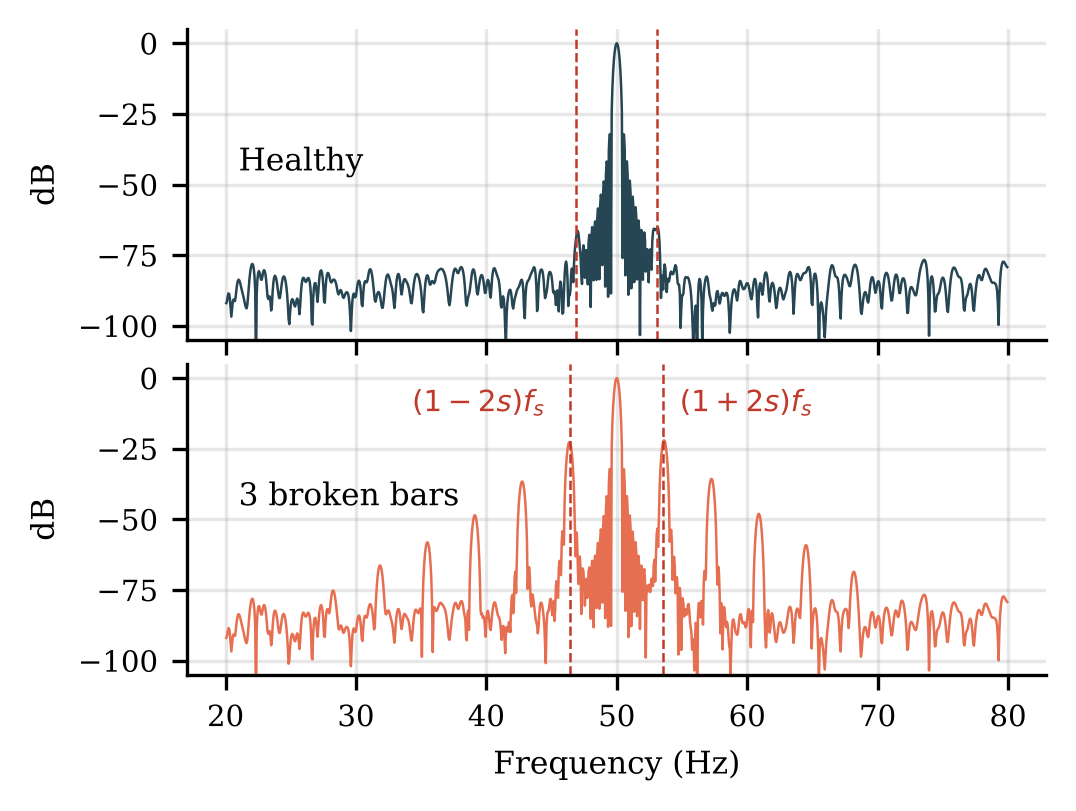
\includegraphics[width=\columnwidth]{spectrum.png}
\caption{Phase-$a$ current spectrum at 80\,\% load: healthy motor (top) and three broken bars (bottom). Dashed lines: theoretical $(1\pm2s)f_s$ sidebands.}
\label{fig:spectrum}
\end{figure}

\begin{figure}[!t]
\centering
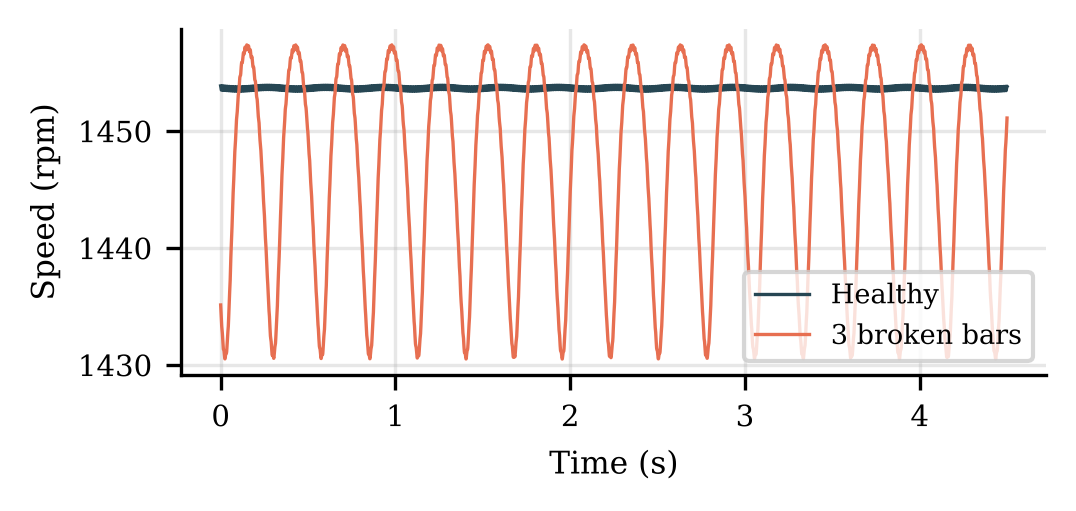
\includegraphics[width=\columnwidth]{speed.png}
\caption{Rotor speed of the healthy motor and of the motor with three broken bars (oscillation at $2sf_s\approx3.5$~Hz).}
\label{fig:speed}
\end{figure}

% ----------------------------------------------------------------------------
\section{Feature Extraction}
From the three currents, the three voltages and the speed, 19 features are computed:
\begin{itemize}
\item \emph{Time domain:} RMS, peak, crest factor, kurtosis and skewness of $i_a$.
\item \emph{Symmetry:} the current unbalance $\max_k|I_k-\bar I|/\bar I$, and the negative-sequence ratios $I_2/I_1$ and $V_2/V_1$ obtained with the Fortescue transform of the fundamental phasors. $V_2/V_1$ separates supply unbalance (high $V_2$) from a winding fault (high $I_2$ with balanced voltages).
\item \emph{Park's vector:} $i_D=\sqrt{2/3}\,i_a-(i_b+i_c)/\sqrt6$ and $i_Q=(i_b-i_c)/\sqrt2$. The features are the eccentricity of the $(i_D,i_Q)$ pattern and the relative ripple of its modulus.
\item \emph{Spectrum} (Hann window, zero-padded FFT): amplitudes in dB relative to the fundamental at $(1\pm2s)f_s$ and $|f_s\pm f_o|$, the third harmonic, the THD, and the energy in the 2--47~Hz and 53--150~Hz bands. The slip $s$ is taken from the speed sensor.
\item \emph{Operating point:} the slip, which tells the network the load level.
\end{itemize}
All features are z-score normalised with the mean and standard deviation of the \emph{training} set only.

\begin{figure}[!t]
\centering
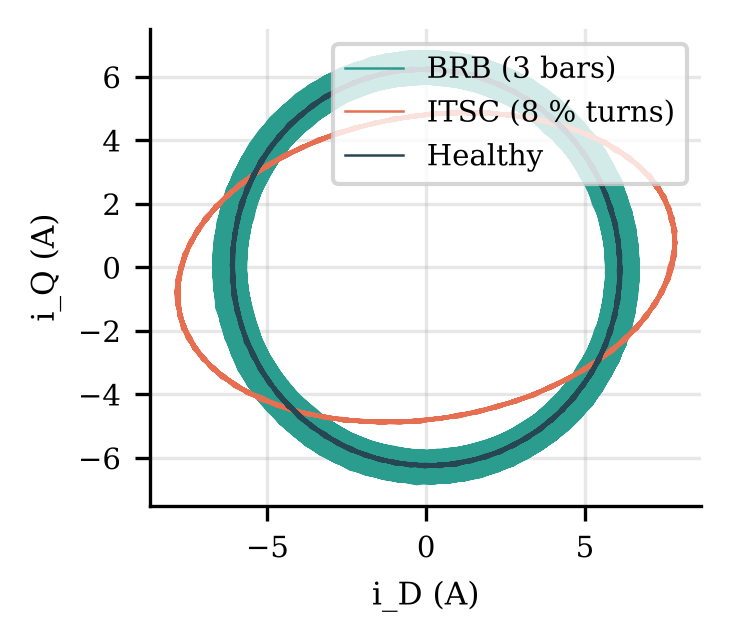
\includegraphics[width=0.62\columnwidth]{park.png}
\caption{Park's vector patterns: healthy (circle), inter-turn short (ellipse) and broken bars (thick ring).}
\label{fig:park}
\end{figure}

% ----------------------------------------------------------------------------
\section{Neural Networks}
All networks are implemented in NumPy without machine-learning libraries, so that each update matches the course equations. A neuron computes $y=\varphi(v)$ with $v=\sum_i w_i x_i-\theta$, where the threshold $\theta$ is a weight applied to a constant input $-1$. The instantaneous cost is $E(n)=\tfrac12\sum_j e_j^2(n)$ with $e_j=y_j^*-y_j$.

\subsection{Single-Layer Networks}
The \emph{Perceptron} \cite{rosenblatt1958} uses a hard limiter and the error-correction rule $\Delta\mathbf{w}=\eta(d-y)\mathbf{x}$, with one neuron per class. \emph{ADALINE} \cite{widrow1960} applies the LMS rule $\Delta\mathbf{w}=\eta\,e\,\mathbf{x}$ to the linear output, before the limiter. Both can only separate classes with hyperplanes.

\subsection{Multilayer Perceptron with Back-Propagation}
The MLP has one hidden layer (15 $\tanh$ neurons) and logistic output neurons. It is trained in sequential mode with back-propagation \cite{rumelhart1986}:
\begin{align}
\delta_j &= e_j\,\varphi_o'(v_j), \qquad \delta_k = \varphi_h'(v_k)\sum_j \delta_j w_{jk},\\
\Delta w(n) &= \eta\,\delta\,y + \alpha\,\Delta w(n-1),
\end{align}
where $\alpha=0$ gives classic BP and $\alpha=0.8$ adds the momentum term. In the \emph{adaptive learning-rate} variant, $\eta$ is multiplied by 1.05 after an epoch that decreases $E$. When $E$ increases by more than 4\,\%, the epoch is rejected, $\eta$ is multiplied by 0.7 and the momentum memory is reset.

\subsection{Levenberg--Marquardt}
In batch mode, the weight vector is updated with \cite{hagan1994}
\begin{equation}
\Delta\mathbf{w} = -\left(\mathbf{J}^{\mathsf T}\mathbf{J}+\mu\mathbf{I}\right)^{-1}\mathbf{J}^{\mathsf T}\mathbf{e},
\end{equation}
where $\mathbf{J}=\partial\mathbf{e}/\partial\mathbf{w}$ is computed analytically and checked by finite differences. $\mu$ is divided by 10 after a successful step and multiplied by 10 after a failed one. LM therefore moves between gradient descent ($\eta\approx1/\mu$) and the Gauss--Newton method.

\subsection{RBF Network}
The RBF network uses $M$ Gaussian neurons $\varphi_j(\mathbf{x})=\exp(-M\|\mathbf{x}-\mathbf{t}_j\|^2/d^2)$, i.e., $\sigma=d/\sqrt{2M}$. The centres $\mathbf{t}_j$ are drawn at random from the training vectors and $d$ is their maximum distance \cite{broomhead1988}. The output weights are obtained in one step with the pseudo-inverse, $\mathbf{w}=\mathbf{G}^{+}\mathbf{y}^*$.

\subsection{Training Protocol}
The data are split, stratified by class, into a \emph{training} set (60\,\%) used to adjust the weights, a \emph{test} set (20\,\%) used for early stopping, and a \emph{validation} set (20\,\%) used only for the final, unbiased evaluation. During training the test error is monitored after every epoch, and the weights at its minimum (point~A, Fig.~\ref{fig:learning}) are kept \cite{prechelt1998}. Default hyper-parameters: $\eta=0.02$, 300 epochs (100 for LM), $\mu_0=0.01$ and $M=40$ centres.

% ----------------------------------------------------------------------------
\section{Results}
\begin{figure*}[t]
\centering
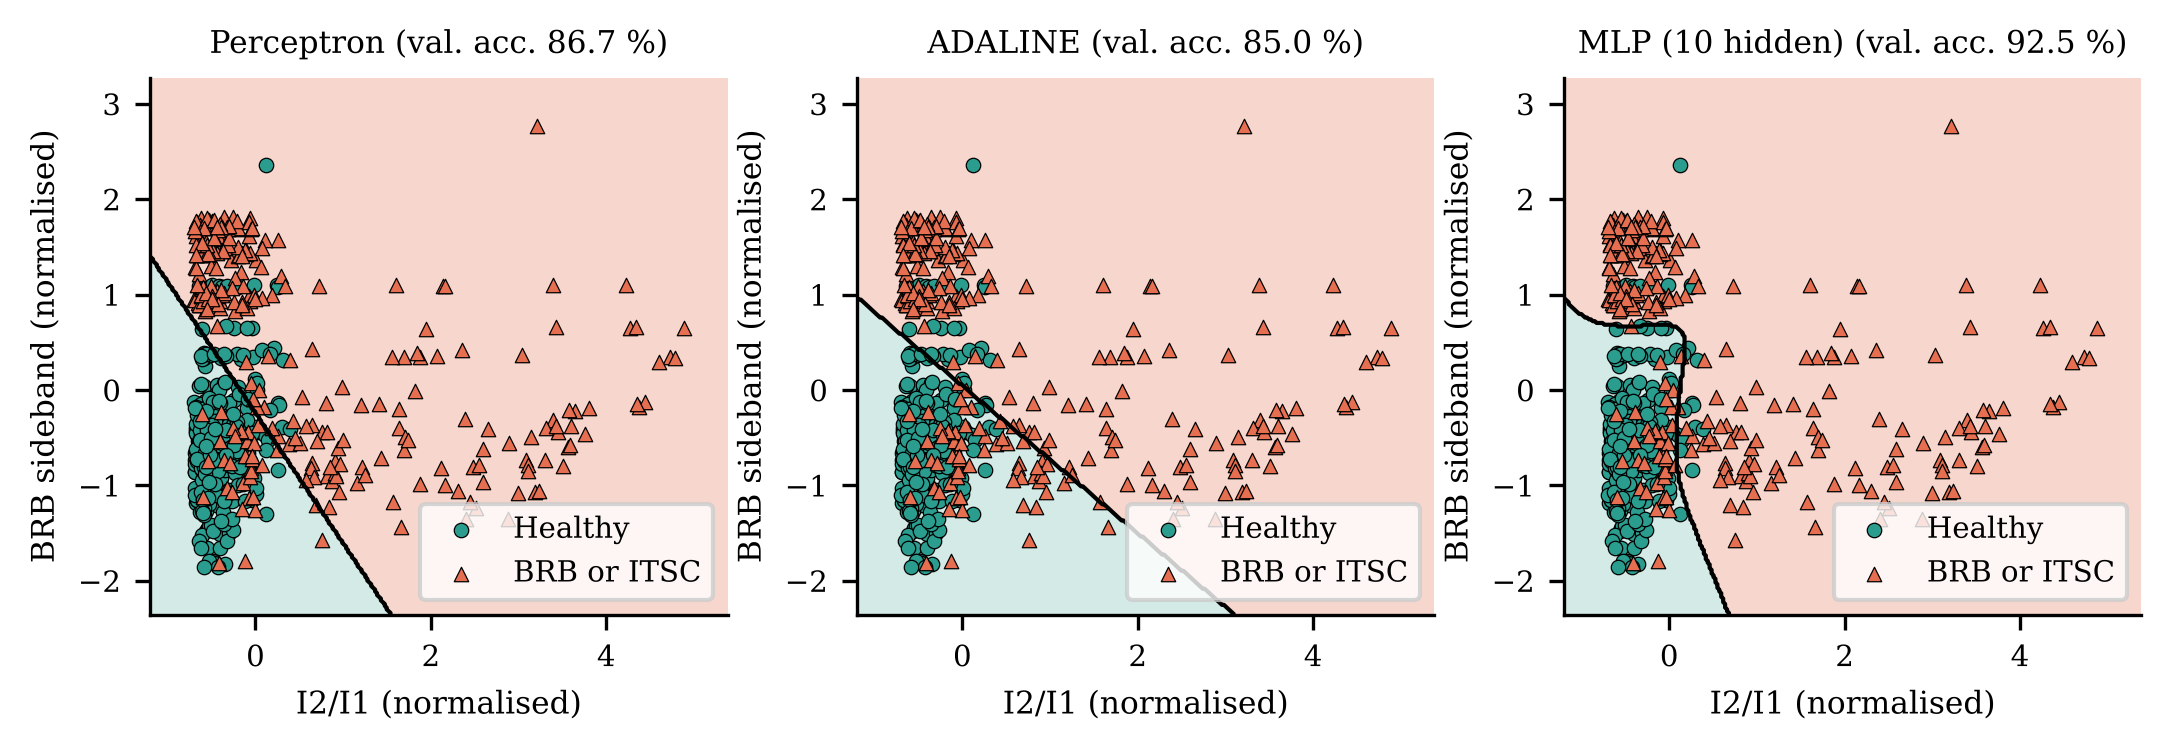
\includegraphics[width=\textwidth]{regions.png}
\caption{Decision regions with two features ($I_2/I_1$ and BRB sideband, normalised). The single-layer networks draw a line; the MLP bends around the healthy corner.}
\label{fig:regions}
\end{figure*}
\subsection{Dataset and Single-Run Comparison}
The dataset contains 1500 motors, 300 per class with the severities balanced. For detection, all healthy motors and an equal number of faulty motors (drawn equally from the four fault classes) are used. Table~\ref{tab:single} reports the validation metrics of one run. A scikit-learn MLP with the same architecture reaches 94.3\,\% (diagnosis), which confirms that the from-scratch implementation is correct.

\begin{table}[!t]
\caption{Validation Results of One Run (Diagnosis: 5 Classes, Detection: 2 Classes)}
\label{tab:single}
\centering\footnotesize
\setlength{\tabcolsep}{3.5pt}
\begin{tabular}{@{}lcccccc@{}}
\toprule
 & \multicolumn{4}{c}{Diagnosis} & \multicolumn{2}{c}{Detection}\\
\cmidrule(lr){2-5}\cmidrule(l){6-7}
Network & Acc.\,\% & F1\,\% & Time (s) & A & Acc.\,\% & Rec.\,\%\\
\midrule
Perceptron     & 93.7 & 93.7 & 2.2  & 75  & 91.7 & 90.0\\
ADALINE        & 91.3 & 91.4 & 1.3  & 69  & 88.3 & 83.3\\
MLP-BP         & \textbf{95.3} & 95.3 & 8.4  & 149 & 91.7 & 88.3\\
MLP-momentum   & 94.3 & 94.4 & 8.7  & 37  & 92.5 & 88.3\\
MLP-adaptive $\eta$ & 94.3 & 94.4 & 8.1 & 52 & 92.5 & 88.3\\
MLP-LM         & \textbf{95.3} & 95.4 & 2.9  & 7   & 91.7 & 90.0\\
RBF ($M{=}40$) & 75.7 & 75.7 & 0.01 & --  & 92.5 & 93.3\\
\bottomrule
\end{tabular}
\end{table}

Momentum and the adaptive learning rate reach point A three to four times earlier than classic BP (epochs 37--52 versus 149). LM reaches it after only 7 iterations and is the fastest MLP. After point A, LM drives the training error towards zero while the test error rises, which is a clear case of over-fitting that early stopping removes. Fig.~\ref{fig:learning} shows the learning curve of classic BP. The confusion matrix (Fig.~\ref{fig:cm}) shows that broken bars are always recognised. Most errors are healthy motors confused with supply unbalance, and inter-turn shorts confused with healthy motors.

\begin{figure}[!t]
\centering
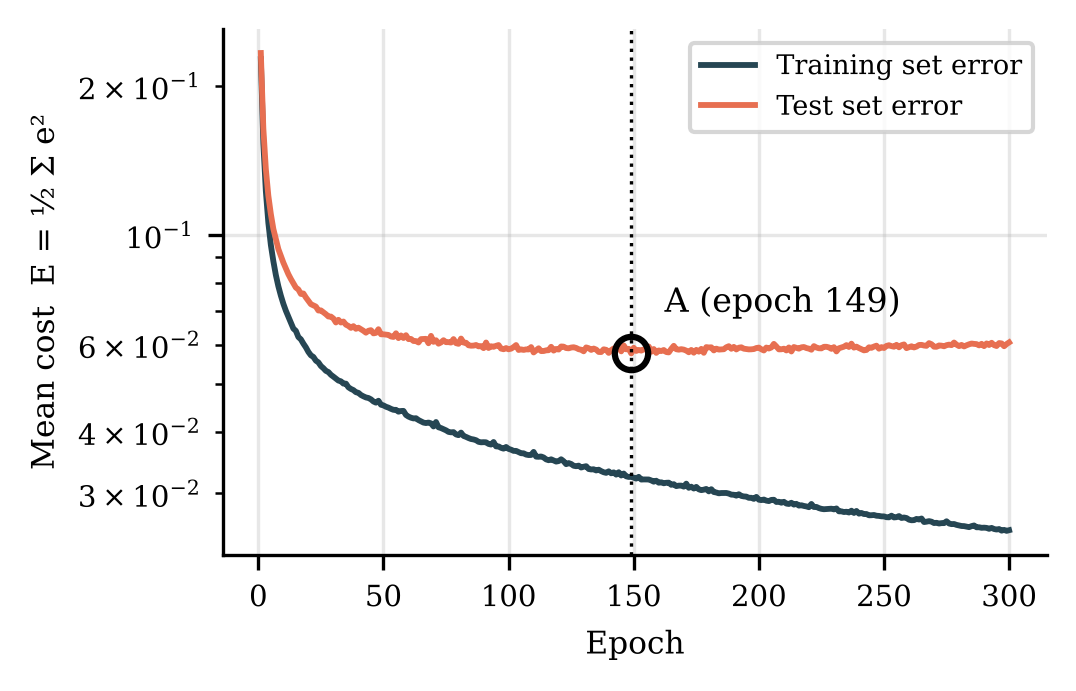
\includegraphics[width=\columnwidth]{learning_A.png}
\caption{Training and test error of MLP-BP (diagnosis). The weights are kept at point A, the minimum of the test error.}
\label{fig:learning}
\end{figure}

\begin{figure}[!t]
\centering
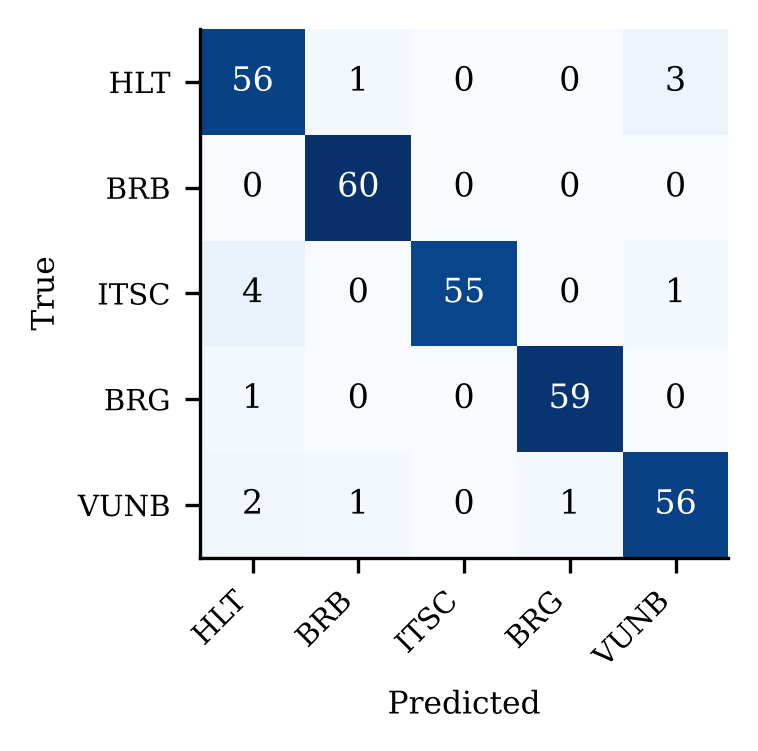
\includegraphics[width=0.7\columnwidth]{cm_mlp.png}
\caption{Confusion matrix of MLP-BP on the validation set (diagnosis).}
\label{fig:cm}
\end{figure}

\begin{figure*}[t]
\centering
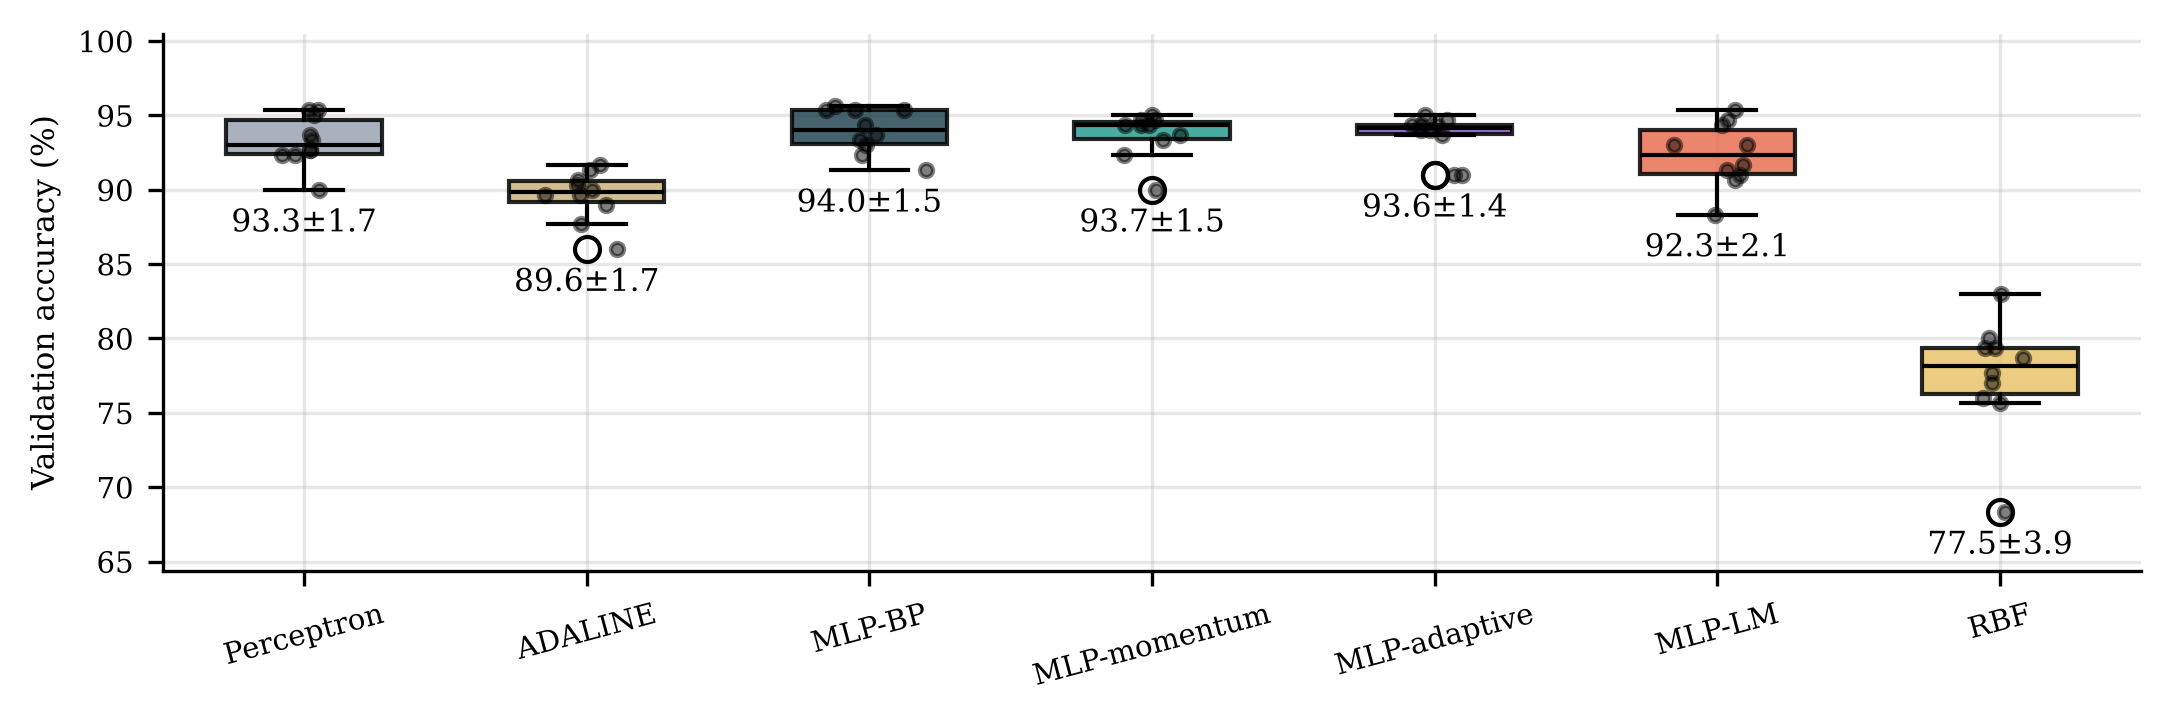
\includegraphics[width=\textwidth]{repeated.png}
\caption{Diagnosis accuracy of the seven networks over ten independent runs (new split and new initial weights each run).}
\label{fig:repeated}
\end{figure*}
\begin{figure*}[t]
\centering
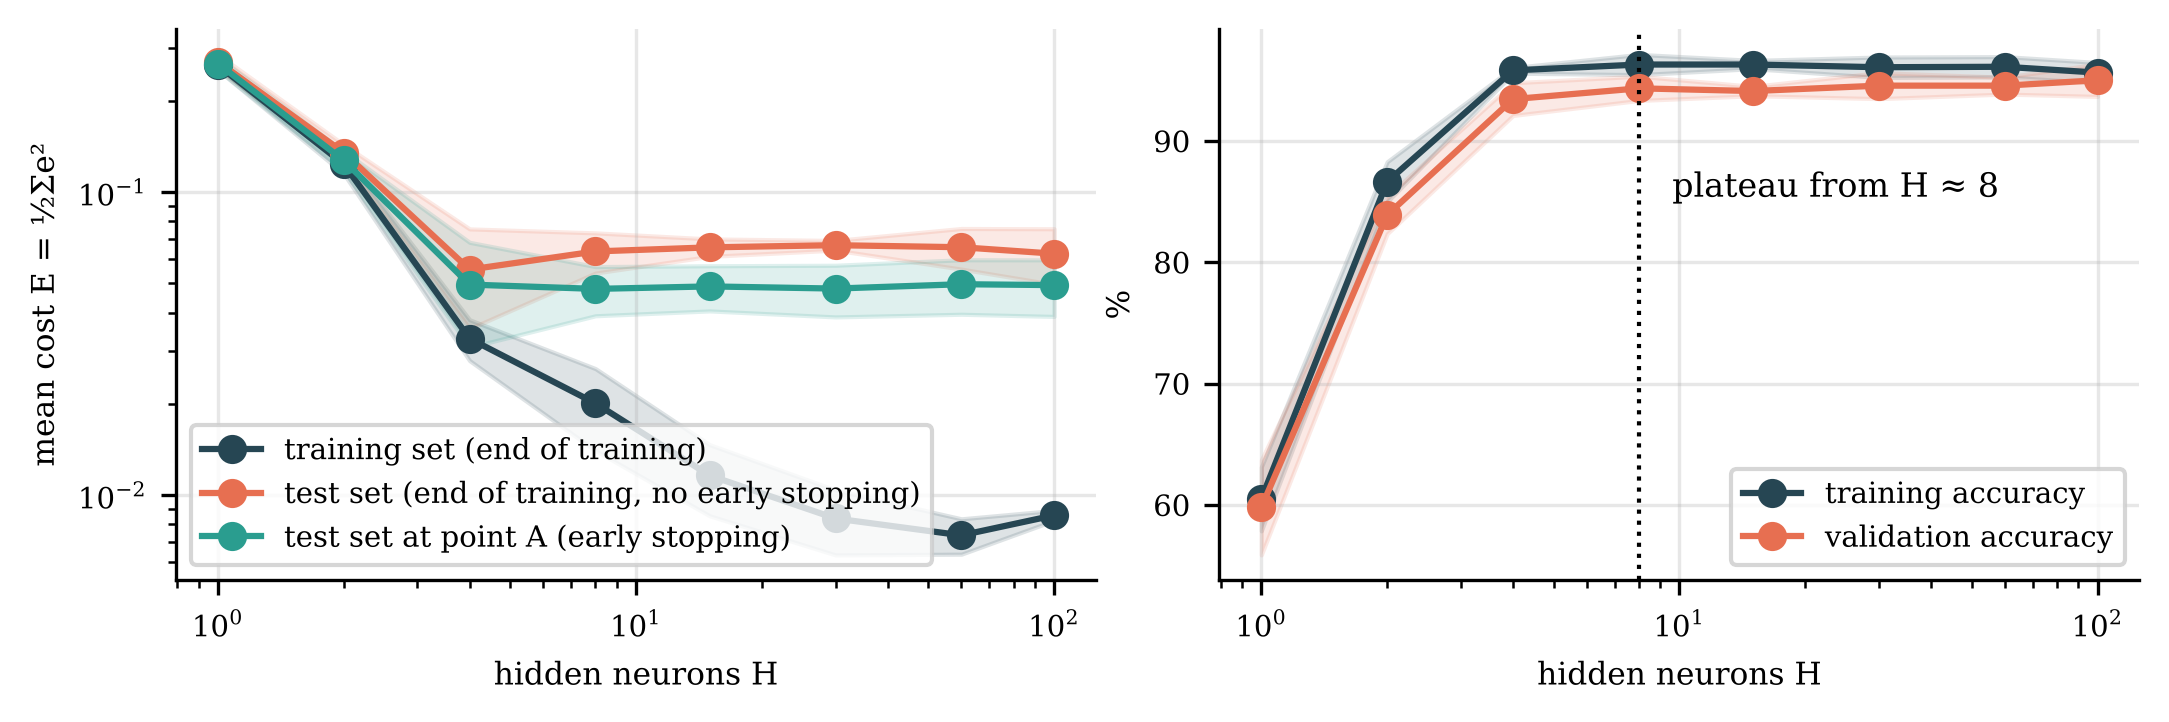
\includegraphics[width=\textwidth]{hidden.png}
\caption{Effect of the number of hidden neurons $H$ (mean and standard deviation of three runs): error (left) and accuracy (right).}
\label{fig:hidden}
\end{figure*}
\subsection{Linear Versus Non-Linear Separation}
With all 19 features the classes are almost linearly separable, which explains the good score of the Perceptron. To isolate the role of the hidden layer, a two-feature detection problem was built: healthy motors versus motors with broken bars or an inter-turn short, described only by $I_2/I_1$ and the lower BRB sideband. The healthy class occupies a corner of the plane, so the faulty region is the union (OR) of two half-planes. A single hyperplane cannot represent this region, while the MLP bends its boundary around the corner (Fig.~\ref{fig:regions}): 92.5\,\% validation accuracy, against 86.7\,\% for the Perceptron and 85.0\,\% for ADALINE.


\subsection{Repeated Runs}
A single run can be lucky, so each network was trained ten times, each time with a new random three-set split and new initial weights (Fig.~\ref{fig:repeated}, Table~\ref{tab:repeated}). MLP-BP has the best mean diagnosis accuracy, $94.0\pm1.5$\,\%. Momentum and adaptive $\eta$ give practically the same accuracy, $93.7$ and $93.6$\,\%. LM is less stable ($92.3\pm2.1$\,\%), because its fast convergence makes it sensitive to the split. The MLPs clearly outperform ADALINE and RBF, but their advantage over the Perceptron ($0.7$ points) is smaller than the run-to-run spread. The single-run ranking of Table~\ref{tab:single} therefore slightly exaggerated the differences.

\begin{table}[!t]
\caption{Mean $\pm$ Standard Deviation Over 10 Runs (Validation Accuracy, \%)}
\label{tab:repeated}
\centering\footnotesize
\begin{tabular}{@{}lccc@{}}
\toprule
Network & Diagnosis & Detection & Time (s)\\
\midrule
Perceptron   & $93.3\pm1.7$ & $90.3\pm2.3$ & 1.7\\
ADALINE      & $89.6\pm1.7$ & $87.0\pm2.1$ & 1.2\\
MLP-BP       & $\mathbf{94.0\pm1.5}$ & $\mathbf{91.6\pm1.3}$ & 7.2\\
MLP-momentum & $93.7\pm1.5$ & $91.3\pm2.1$ & 7.1\\
MLP-adaptive $\eta$ & $93.6\pm1.4$ & $91.2\pm1.7$ & 7.0\\
MLP-LM       & $92.3\pm2.1$ & $91.5\pm2.2$ & 2.7\\
RBF          & $77.5\pm3.9$ & $87.5\pm3.4$ & 0.01\\
\bottomrule
\end{tabular}
\end{table}


\subsection{Robustness}
A fresh pool of 500 motors, never used for training, was simulated and diagnosed by the saved networks.

\emph{Severity and load} (1\,\% noise, Fig.~\ref{fig:severity}): MLP-BP recognises incipient faults (severity~1) in 89\,\% of cases and medium or severe faults in 100\,\%. Almost all errors therefore come from the smallest faults. Accuracy stays between 92\,\% and 98\,\% in every load band from 30 to 110\,\%.

\emph{Sensor noise} (Fig.~\ref{fig:noise}): within the training range (0.25--2\,\%) the MLPs keep about 90--95\,\%. Beyond it they degrade quickly: at 5\,\% noise MLP-BP falls to 31\,\%, while the linear ADALINE keeps 65\,\%. The MLP has learned sharp boundaries tuned to the training conditions, so the training data must contain the noise level of the real sensors.

\begin{figure}[!t]
\centering
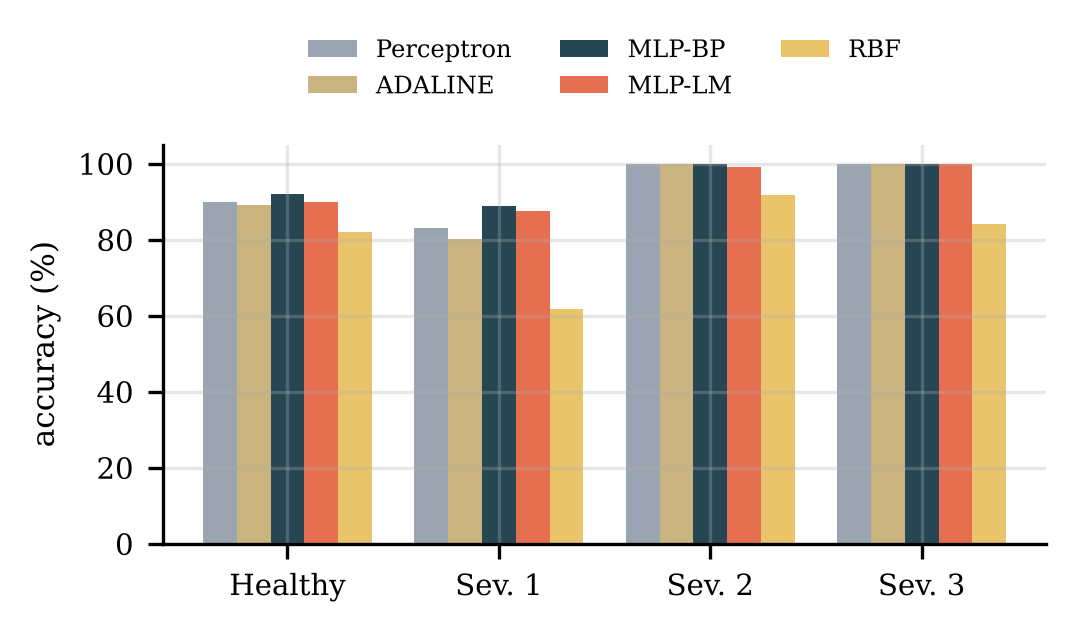
\includegraphics[width=\columnwidth]{severity.png}
\caption{Diagnosis accuracy versus fault severity on 500 unseen motors (1\,\% noise).}
\label{fig:severity}
\end{figure}

\begin{figure}[!t]
\centering
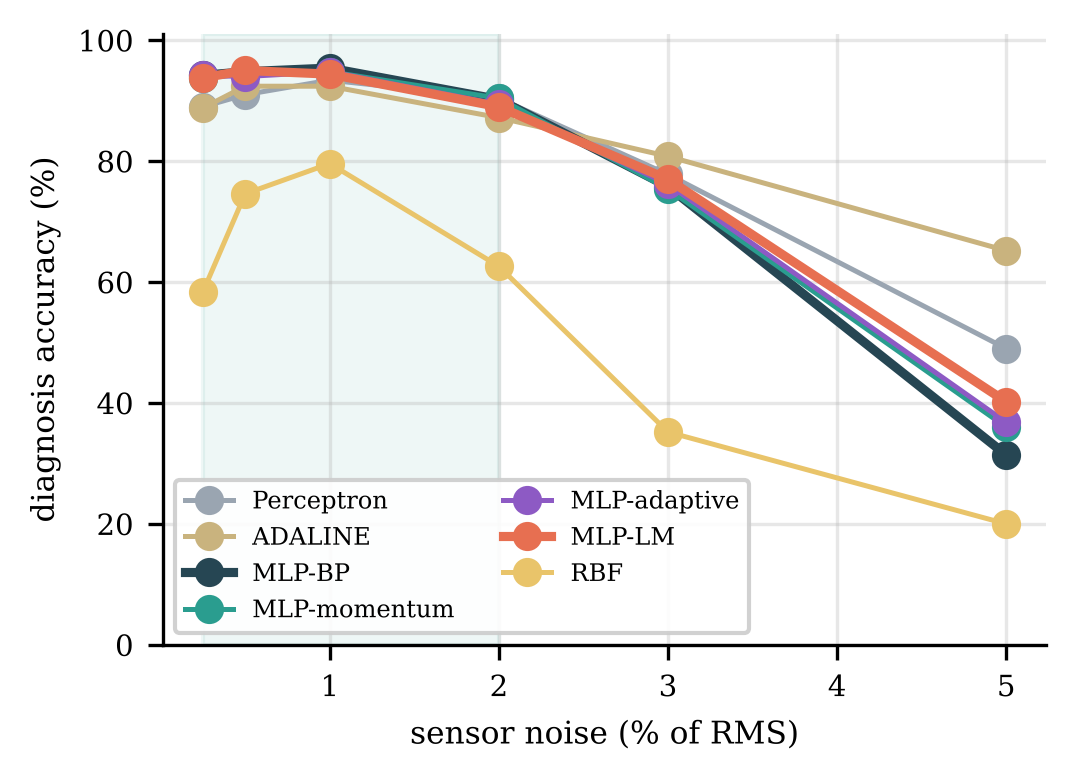
\includegraphics[width=\columnwidth]{noise.png}
\caption{Diagnosis accuracy versus sensor noise on 500 unseen motors. Shaded band: noise range seen during training.}
\label{fig:noise}
\end{figure}

\subsection{Size of the Hidden Layer}
The MLP was trained with $H=1$ to $100$ hidden neurons, with three runs per size (Fig.~\ref{fig:hidden}). With one or two neurons the network under-fits (60\,\% and 84\,\%). From $H\approx8$ the validation accuracy reaches a plateau of about 95\,\%. Larger networks keep lowering the training error, while their end-of-training test error rises slightly (over-fitting). Early stopping at point A keeps them as accurate as the smaller networks.


% ----------------------------------------------------------------------------
\section{Discussion}
\emph{MLP versus RBF.} The sigmoid neurons of the MLP respond globally, since each one splits the whole input space with a hyperplane. The Gaussian neurons of the RBF network respond only near their centre. With fixed random centres and a single width set by the largest distance, 40 centres cannot cover a 19-dimensional space, and the result depends strongly on which centres are drawn ($77.5\pm3.9$\,\%). RBF training is, however, about a thousand times faster, because it reduces to one linear least-squares solution with no local minima. Selecting the centres with a supervised method or with clustering would be the natural improvement.

\emph{Role of the features.} The physics-based features make the problem almost linear, which is why the Perceptron performs well. The hidden layer becomes decisive when the information is spread over fewer or less direct features (Fig.~\ref{fig:regions}).

\emph{Limitations.} The data are simulated. The inter-turn short neglects the circulating current in the shorted loop. The bearing fault is modelled as a torque oscillation, without a vibration sensor. Saturation and slot harmonics are ignored. The networks would therefore have to be re-trained or fine-tuned on measured currents, for example from the Paderborn bearing benchmark \cite{lessmeier2016} or from a laboratory test bench.

% ----------------------------------------------------------------------------
\section{Conclusion}
A complete, simulation-based fault detection and diagnosis system for induction motors was developed, from a physical motor model with injected faults to MCSA features and seven neural networks implemented from scratch. The back-propagation MLP is the most accurate and most reliable network ($94.0\pm1.5$\,\% over ten runs for five classes). It detects 89\,\% of incipient faults and all medium and severe faults on unseen motors, while Levenberg--Marquardt offers the fastest convergence. The study also shows the value of repeated runs, of early stopping and of training under realistic noise. Future work includes validation on measured data, estimation of the fault severity, and prognosis of the remaining useful life.

\section*{Acknowledgment}
The authors thank Prof. Hadi Y. Kanaan for his guidance in the course \emph{AI-Based Control Systems}. The code, data and interactive application are available from the authors.

\begin{thebibliography}{99}
\footnotesize
\bibitem{nandi2005} S. Nandi, H. A. Toliyat, and X. Li, ``Condition monitoring and fault diagnosis of electrical motors---A review,'' \emph{IEEE Trans. Energy Convers.}, vol. 20, no. 4, pp. 719--729, Dec. 2005.
\bibitem{benbouzid2000} M. E. H. Benbouzid, ``A review of induction motors signature analysis as a medium for faults detection,'' \emph{IEEE Trans. Ind. Electron.}, vol. 47, no. 5, pp. 984--993, Oct. 2000.
\bibitem{thomson2001} W. T. Thomson and M. Fenger, ``Current signature analysis to detect induction motor faults,'' \emph{IEEE Ind. Appl. Mag.}, vol. 7, no. 4, pp. 26--34, Jul./Aug. 2001.
\bibitem{haykin1999} S. Haykin, \emph{Neural Networks: A Comprehensive Foundation}, 2nd ed. Upper Saddle River, NJ, USA: Prentice Hall, 1999.
\bibitem{goode1995} P. V. Goode and M.-Y. Chow, ``Using a neural/fuzzy system to extract heuristic knowledge of incipient faults in induction motors: Part I---Methodology,'' \emph{IEEE Trans. Ind. Electron.}, vol. 42, no. 2, pp. 131--138, Apr. 1995.
\bibitem{krause2002} P. C. Krause, O. Wasynczuk, and S. D. Sudhoff, \emph{Analysis of Electric Machinery and Drive Systems}, 2nd ed. Piscataway, NJ, USA: Wiley-IEEE Press, 2002.
\bibitem{bellini2008} A. Bellini, F. Filippetti, C. Tassoni, and G.-A. Capolino, ``Advances in diagnostic techniques for induction machines,'' \emph{IEEE Trans. Ind. Electron.}, vol. 55, no. 12, pp. 4109--4126, Dec. 2008.
\bibitem{tallam2002} R. M. Tallam, T. G. Habetler, and R. G. Harley, ``Transient model for induction machines with stator winding turn faults,'' \emph{IEEE Trans. Ind. Appl.}, vol. 38, no. 3, pp. 632--637, May/Jun. 2002.
\bibitem{schoen1995} R. R. Schoen, T. G. Habetler, F. Kamran, and R. G. Bartheld, ``Motor bearing damage detection using stator current monitoring,'' \emph{IEEE Trans. Ind. Appl.}, vol. 31, no. 6, pp. 1274--1279, Nov./Dec. 1995.
\bibitem{cardoso1999} A. J. M. Cardoso, S. M. A. Cruz, and D. S. B. Fonseca, ``Inter-turn stator winding fault diagnosis in three-phase induction motors, by Park's vector approach,'' \emph{IEEE Trans. Energy Convers.}, vol. 14, no. 3, pp. 595--598, Sep. 1999.
\bibitem{rosenblatt1958} F. Rosenblatt, ``The perceptron: A probabilistic model for information storage and organization in the brain,'' \emph{Psychol. Rev.}, vol. 65, no. 6, pp. 386--408, 1958.
\bibitem{widrow1960} B. Widrow and M. E. Hoff, ``Adaptive switching circuits,'' in \emph{IRE WESCON Conv. Rec.}, pt. 4, 1960, pp. 96--104.
\bibitem{rumelhart1986} D. E. Rumelhart, G. E. Hinton, and R. J. Williams, ``Learning representations by back-propagating errors,'' \emph{Nature}, vol. 323, pp. 533--536, Oct. 1986.
\bibitem{hagan1994} M. T. Hagan and M. B. Menhaj, ``Training feedforward networks with the Marquardt algorithm,'' \emph{IEEE Trans. Neural Netw.}, vol. 5, no. 6, pp. 989--993, Nov. 1994.
\bibitem{broomhead1988} D. S. Broomhead and D. Lowe, ``Multivariable functional interpolation and adaptive networks,'' \emph{Complex Syst.}, vol. 2, pp. 321--355, 1988.
\bibitem{prechelt1998} L. Prechelt, ``Early stopping---But when?'' in \emph{Neural Networks: Tricks of the Trade}, G. B. Orr and K.-R. M\"uller, Eds. Berlin, Germany: Springer, 1998, pp. 55--69.
\bibitem{lessmeier2016} C. Lessmeier, J. K. Kimotho, D. Zimmer, and W. Sextro, ``Condition monitoring of bearing damage in electromechanical drive systems by using motor current signals of electric motors: A benchmark data set for data-driven classification,'' in \emph{Proc. Eur. Conf. PHM Soc.}, 2016.
\end{thebibliography}

\end{document}
